\documentclass[tikz,border=7pt]{standalone}
\usepackage{amsmath,pgfplots}
\pgfplotsset{compat=1.18}
\usepgfplotslibrary{groupplots}
\begin{document}
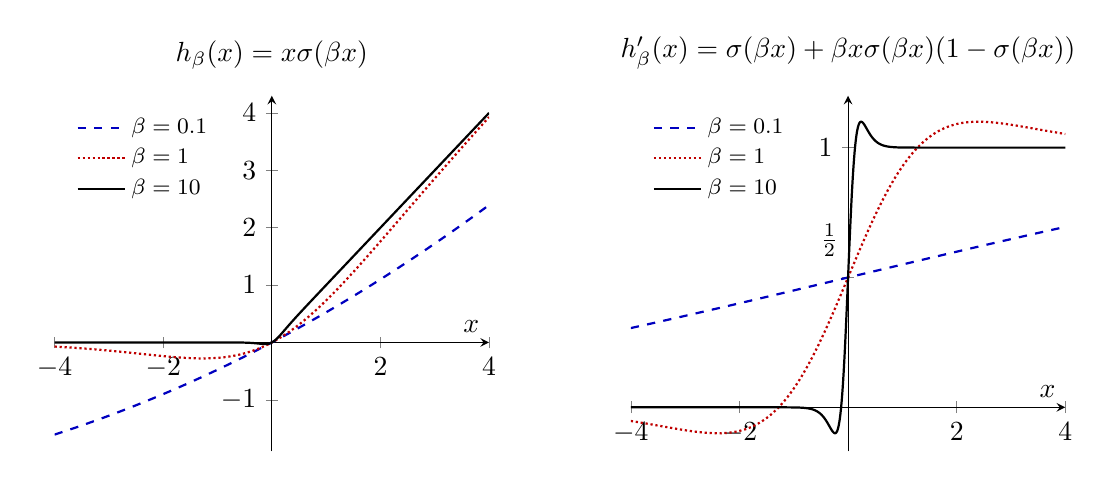
\begin{tikzpicture}
\begin{groupplot}[group style={group size=2 by 1,horizontal sep=1.8cm},
width=7.1cm,height=6.1cm,xmin=-4,xmax=4,domain=-4:4,samples=801,
axis lines=middle,xlabel={$x$},xtick={-4,-2,0,2,4},
legend cell align=left,legend style={draw=none,font=\footnotesize},
every axis plot/.append style={thick}]
\nextgroupplot[ymin=-1.9,ymax=4.3,ytick={-1,0,1,2,3,4},title={$h_\beta(x)=x\sigma(\beta x)$},
legend pos=north west]
\addplot[blue!75!black,dashed] {x/(1+exp(-.1*x))};
\addlegendentry{$\beta=0.1$}
\addplot[red!75!black,densely dotted] {x/(1+exp(-x))};
\addlegendentry{$\beta=1$}
\addplot[black,solid] {x/(1+exp(-10*x))};
\addlegendentry{$\beta=10$}
\nextgroupplot[ymin=-.17,ymax=1.2,ytick={0,.5,1},yticklabels={$0$,{},$1$},
title={$h'_\beta(x)=\sigma(\beta x)+\beta x\sigma(\beta x)(1-\sigma(\beta x))$},
legend pos=north west]
\addplot[blue!75!black,dashed] {1/(1+exp(-.1*x))+.1*x*exp(-.1*x)/(1+exp(-.1*x))^2};
\addlegendentry{$\beta=0.1$}
\addplot[red!75!black,densely dotted] {1/(1+exp(-x))+x*exp(-x)/(1+exp(-x))^2};
\addlegendentry{$\beta=1$}
\addplot[black,solid] {1/(1+exp(-10*x))+10*x*exp(-10*x)/(1+exp(-10*x))^2};
\addlegendentry{$\beta=10$}
\node[above left,yshift=4pt] at (axis cs:0,.5) {$\frac12$};
\end{groupplot}
\end{tikzpicture}
\end{document}
